\documentclass[main.tex]{subfiles} % Subfile-Class


% ============================================================================== %
%                            Subfile document                                    %
% ============================================================================== %

\begin{document}

% Template

\subsubsection{Sensorik Strecken Rückverfolgung}

Der Algorithmus setzt voraus, dass der Roboter zu jedem Zeitpunkt seine
Orientierung als absoluten Winkel vom Startpunkt kennt und die zurückgelegte
Strecke messen kann. In diesem Abschnitt wird beschrieben, wie der Roboter
diese Informationen erhält. Abbildung~\ref{fig:Blockschaltbild_StreckenTracken}
zeigt schematisch, wie diese Funktion implementiert ist. In der folgenden
Beschreibung wird dieses Schema noch einmal erläutert.

\begin{figure}[H]
    \centering
    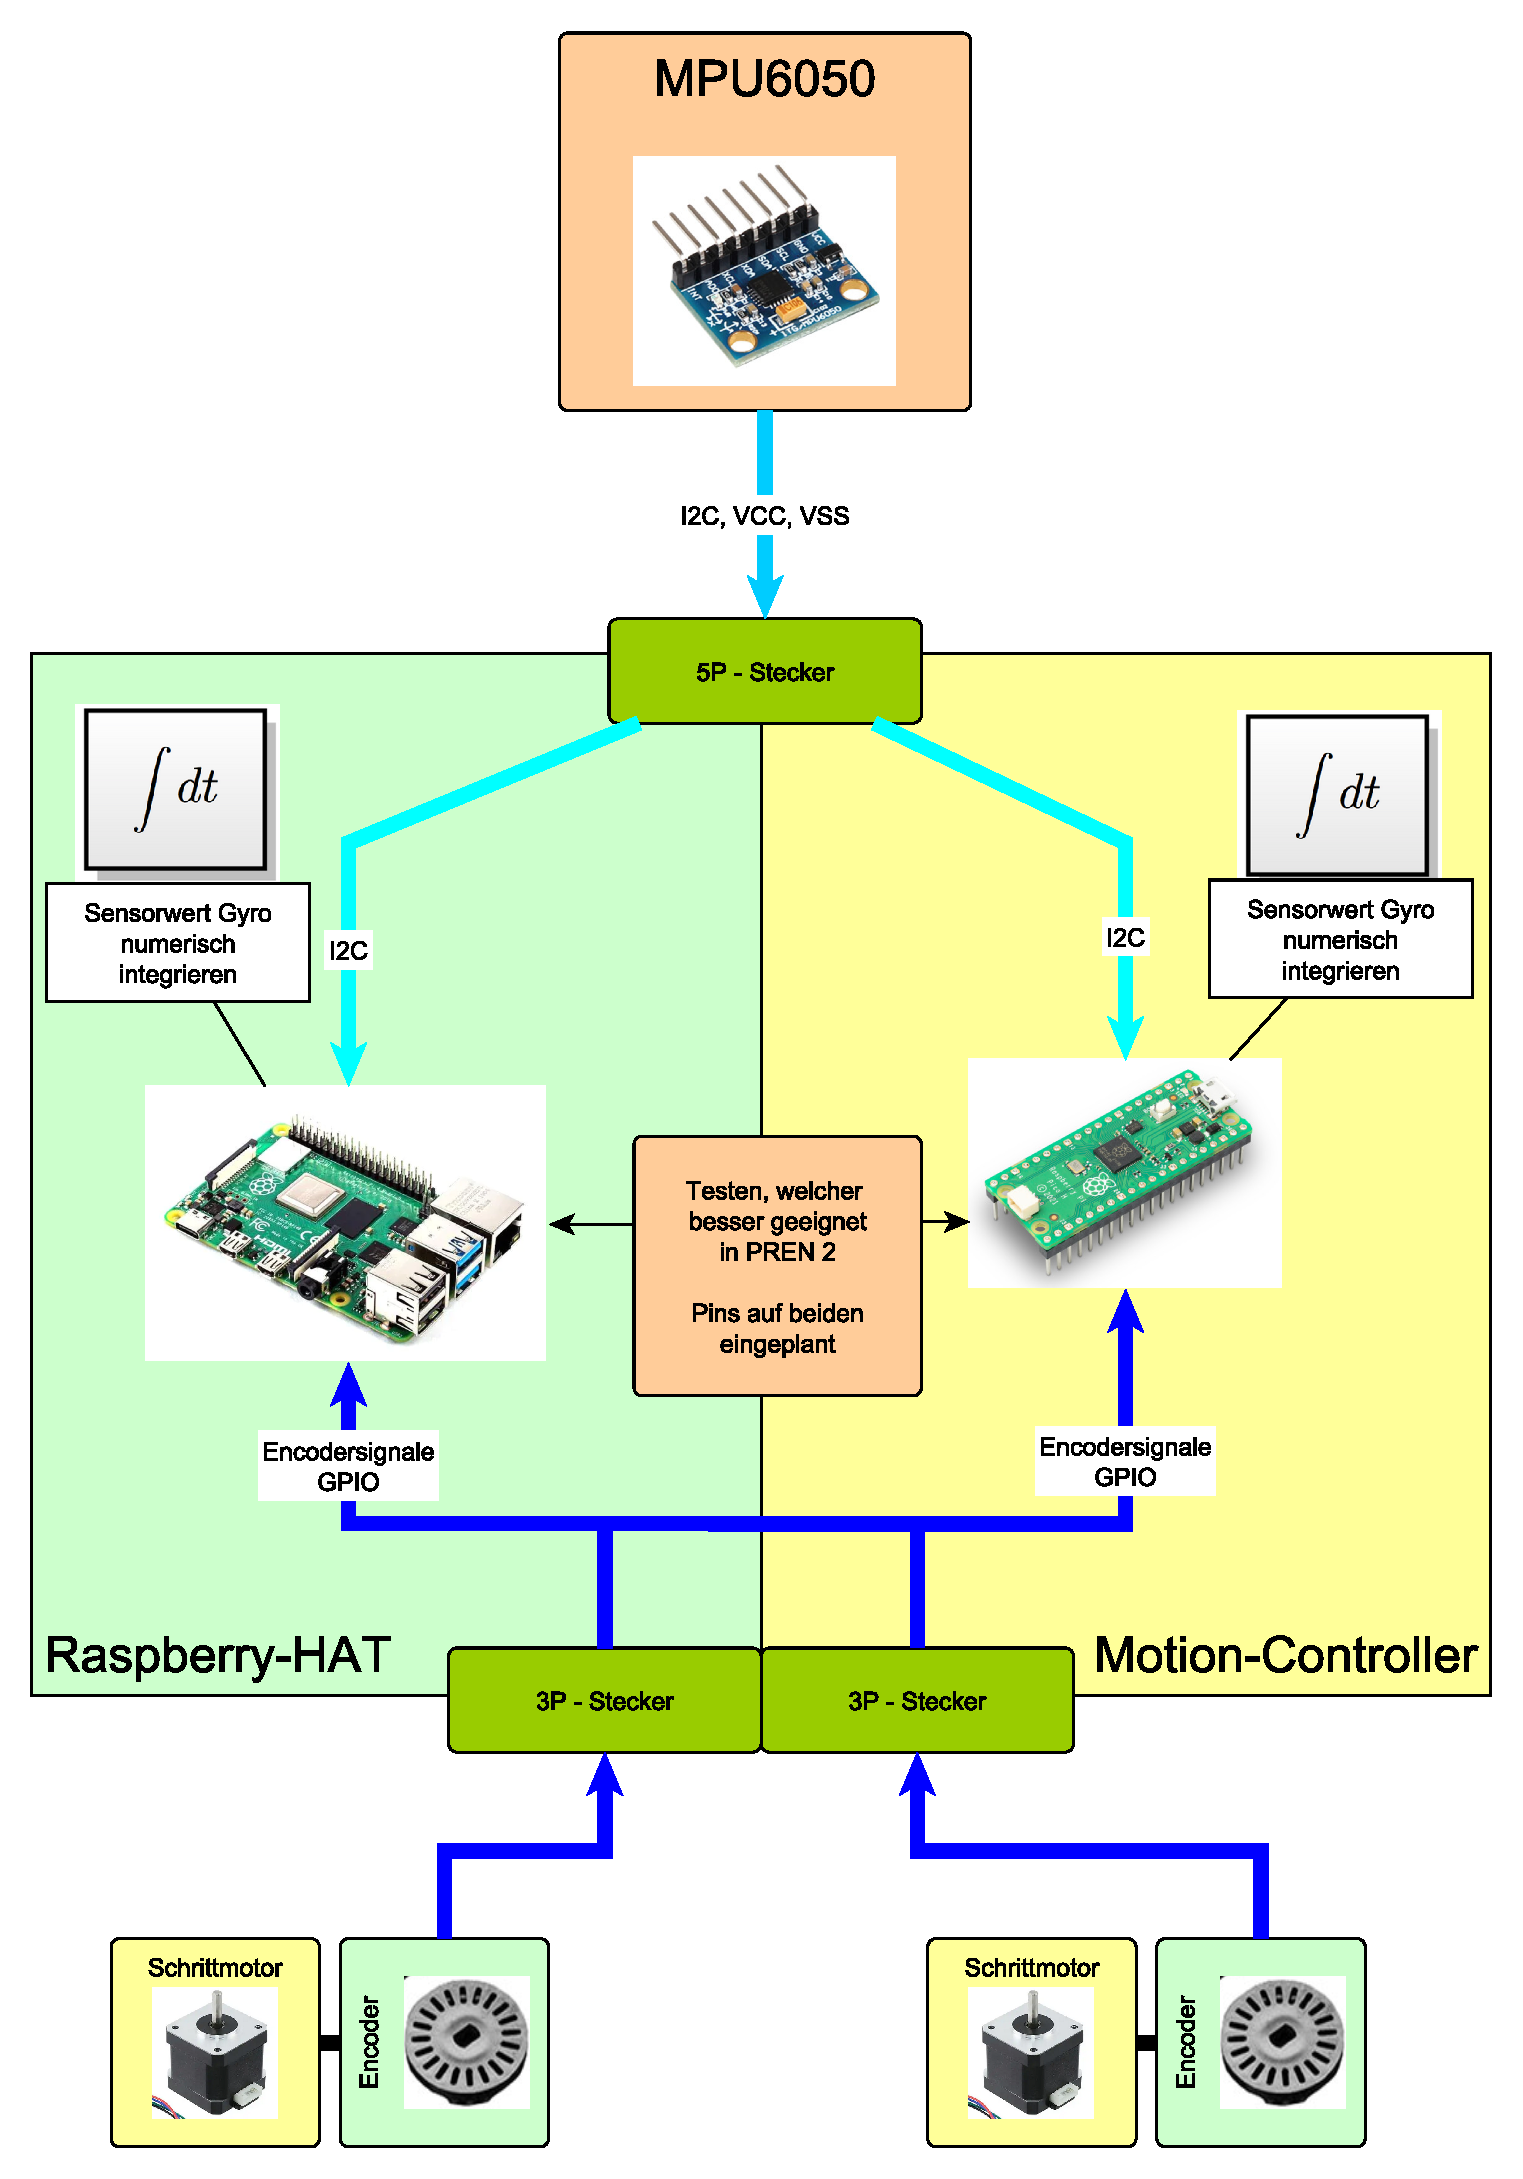
\includegraphics[width=0.75\textwidth]{./fig_Strecke_Tracken/Topologie_MPU6050.pdf}
    \caption{Blockschaltbild Sensorik Streckenrückverfolgung}~\label{fig:Blockschaltbild_StreckenTracken}
\end{figure}

\paragraph{Winkelerfassung}
Der Winkel des Fahrzeugs wird, wie in Anhang~\ref{appendix:Strecke_Tracken}
beschrieben, mit einem Gyroskop gemessen. Dieses erfasst zu jedem Zeitpunkt die
Änderungsrate des aktuellen Winkels und integriert diese alle $25\mu s$
numerisch. Dies ermöglicht eine sehr genaue Aussage über die aktuelle
Orientierung des Roboters.

Mangels Echtzeitfähigkeit ist nicht sicher, ob der Raspberry Pi in der Lage
ist, das Gyroskop ausreichend genau und häufig auszulesen. Daher ist sowohl auf
dem Antriebscontroller als auch auf dem Raspberry-HAT ein entsprechender
Steckplatz vorgesehen, um dies im Nachfolgemodul PREN2 zu testen.

\paragraph{Fahrstrecke} Wie in der Konzeption beschrieben, wird die zurückgelegte Wegstrecke des
Roboters mit Hilfe eines Encoders erfasst. Die verwendete Lochscheibe hat 36
Löcher, was einer Auflösung von 10 Grad pro Schritt entspricht. Die Abmessungen
der Löcher wurden anhand der Herstellerangaben aus dem entsprechenden
Datenblatt festgelegt. Laut Hersteller beträgt die minimale Erfassungsgrösse
1,8 x 0,8 mm, weshalb Löcher mit den Abmessungen 1,8 x 1,6 mm gewählt wurden
(siehe Abbildung~\ref{fig:Lochscheibe_Vermasst}).

Sollte sich während der Tests in PREN 2 herausstellen, dass die Auflösung nicht
ausreicht, könnte der Durchmesser der Lochscheibe vergrössert werden, um bei
gleicher Lochgrösse mehr Löcher pro Umdrehung unterzubringen.

\begin{figure}[H]
    \centering
    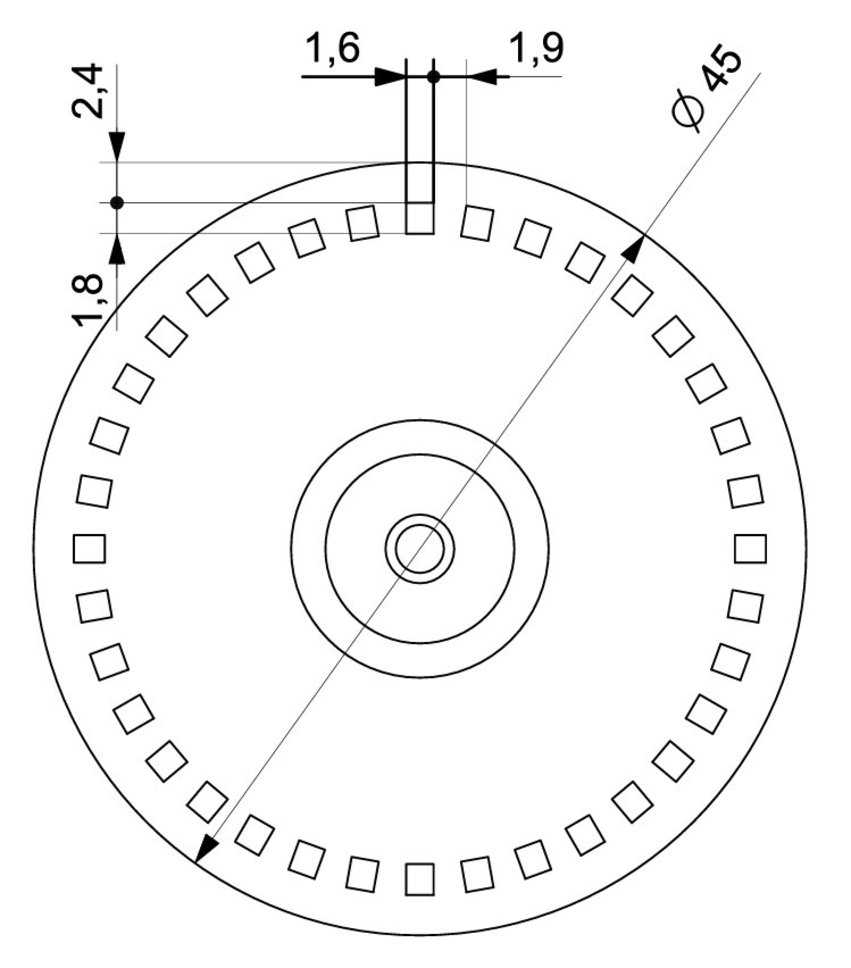
\includegraphics[width=0.5\textwidth]{./fig_Strecke_Tracken/Encoderscheibe_Vermasst.pdf}
    \caption{Masse der Lochscheibe}~\label{fig:Lochscheibe_Vermasst}
\end{figure}

In einem zweiten Versuch soll im Folgemodul PREN2 getestet werden, ob es
ausreicht, für diese Referenz die vom Schrittmotortreiber zurückgelegten
Schritte zu verwenden. Dieser Versuch kann jedoch erst nach dem Bau eines
ersten Roboters mit ausreichender Aussagekraft durchgeführt werden.

\end{document}